% Options for packages loaded elsewhere
\PassOptionsToPackage{unicode}{hyperref}
\PassOptionsToPackage{hyphens}{url}
%
\documentclass[
]{book}
\usepackage{lmodern}
\usepackage{amsmath}
\usepackage{ifxetex,ifluatex}
\ifnum 0\ifxetex 1\fi\ifluatex 1\fi=0 % if pdftex
  \usepackage[T1]{fontenc}
  \usepackage[utf8]{inputenc}
  \usepackage{textcomp} % provide euro and other symbols
  \usepackage{amssymb}
\else % if luatex or xetex
  \usepackage{unicode-math}
  \defaultfontfeatures{Scale=MatchLowercase}
  \defaultfontfeatures[\rmfamily]{Ligatures=TeX,Scale=1}
\fi
% Use upquote if available, for straight quotes in verbatim environments
\IfFileExists{upquote.sty}{\usepackage{upquote}}{}
\IfFileExists{microtype.sty}{% use microtype if available
  \usepackage[]{microtype}
  \UseMicrotypeSet[protrusion]{basicmath} % disable protrusion for tt fonts
}{}
\makeatletter
\@ifundefined{KOMAClassName}{% if non-KOMA class
  \IfFileExists{parskip.sty}{%
    \usepackage{parskip}
  }{% else
    \setlength{\parindent}{0pt}
    \setlength{\parskip}{6pt plus 2pt minus 1pt}}
}{% if KOMA class
  \KOMAoptions{parskip=half}}
\makeatother
\usepackage{xcolor}
\IfFileExists{xurl.sty}{\usepackage{xurl}}{} % add URL line breaks if available
\IfFileExists{bookmark.sty}{\usepackage{bookmark}}{\usepackage{hyperref}}
\hypersetup{
  pdftitle={Comparing AI and Hand Counts of Deer},
  pdfauthor={Courtney Check},
  hidelinks,
  pdfcreator={LaTeX via pandoc}}
\urlstyle{same} % disable monospaced font for URLs
\usepackage{color}
\usepackage{fancyvrb}
\newcommand{\VerbBar}{|}
\newcommand{\VERB}{\Verb[commandchars=\\\{\}]}
\DefineVerbatimEnvironment{Highlighting}{Verbatim}{commandchars=\\\{\}}
% Add ',fontsize=\small' for more characters per line
\usepackage{framed}
\definecolor{shadecolor}{RGB}{248,248,248}
\newenvironment{Shaded}{\begin{snugshade}}{\end{snugshade}}
\newcommand{\AlertTok}[1]{\textcolor[rgb]{0.94,0.16,0.16}{#1}}
\newcommand{\AnnotationTok}[1]{\textcolor[rgb]{0.56,0.35,0.01}{\textbf{\textit{#1}}}}
\newcommand{\AttributeTok}[1]{\textcolor[rgb]{0.77,0.63,0.00}{#1}}
\newcommand{\BaseNTok}[1]{\textcolor[rgb]{0.00,0.00,0.81}{#1}}
\newcommand{\BuiltInTok}[1]{#1}
\newcommand{\CharTok}[1]{\textcolor[rgb]{0.31,0.60,0.02}{#1}}
\newcommand{\CommentTok}[1]{\textcolor[rgb]{0.56,0.35,0.01}{\textit{#1}}}
\newcommand{\CommentVarTok}[1]{\textcolor[rgb]{0.56,0.35,0.01}{\textbf{\textit{#1}}}}
\newcommand{\ConstantTok}[1]{\textcolor[rgb]{0.00,0.00,0.00}{#1}}
\newcommand{\ControlFlowTok}[1]{\textcolor[rgb]{0.13,0.29,0.53}{\textbf{#1}}}
\newcommand{\DataTypeTok}[1]{\textcolor[rgb]{0.13,0.29,0.53}{#1}}
\newcommand{\DecValTok}[1]{\textcolor[rgb]{0.00,0.00,0.81}{#1}}
\newcommand{\DocumentationTok}[1]{\textcolor[rgb]{0.56,0.35,0.01}{\textbf{\textit{#1}}}}
\newcommand{\ErrorTok}[1]{\textcolor[rgb]{0.64,0.00,0.00}{\textbf{#1}}}
\newcommand{\ExtensionTok}[1]{#1}
\newcommand{\FloatTok}[1]{\textcolor[rgb]{0.00,0.00,0.81}{#1}}
\newcommand{\FunctionTok}[1]{\textcolor[rgb]{0.00,0.00,0.00}{#1}}
\newcommand{\ImportTok}[1]{#1}
\newcommand{\InformationTok}[1]{\textcolor[rgb]{0.56,0.35,0.01}{\textbf{\textit{#1}}}}
\newcommand{\KeywordTok}[1]{\textcolor[rgb]{0.13,0.29,0.53}{\textbf{#1}}}
\newcommand{\NormalTok}[1]{#1}
\newcommand{\OperatorTok}[1]{\textcolor[rgb]{0.81,0.36,0.00}{\textbf{#1}}}
\newcommand{\OtherTok}[1]{\textcolor[rgb]{0.56,0.35,0.01}{#1}}
\newcommand{\PreprocessorTok}[1]{\textcolor[rgb]{0.56,0.35,0.01}{\textit{#1}}}
\newcommand{\RegionMarkerTok}[1]{#1}
\newcommand{\SpecialCharTok}[1]{\textcolor[rgb]{0.00,0.00,0.00}{#1}}
\newcommand{\SpecialStringTok}[1]{\textcolor[rgb]{0.31,0.60,0.02}{#1}}
\newcommand{\StringTok}[1]{\textcolor[rgb]{0.31,0.60,0.02}{#1}}
\newcommand{\VariableTok}[1]{\textcolor[rgb]{0.00,0.00,0.00}{#1}}
\newcommand{\VerbatimStringTok}[1]{\textcolor[rgb]{0.31,0.60,0.02}{#1}}
\newcommand{\WarningTok}[1]{\textcolor[rgb]{0.56,0.35,0.01}{\textbf{\textit{#1}}}}
\usepackage{longtable,booktabs}
\usepackage{calc} % for calculating minipage widths
% Correct order of tables after \paragraph or \subparagraph
\usepackage{etoolbox}
\makeatletter
\patchcmd\longtable{\par}{\if@noskipsec\mbox{}\fi\par}{}{}
\makeatother
% Allow footnotes in longtable head/foot
\IfFileExists{footnotehyper.sty}{\usepackage{footnotehyper}}{\usepackage{footnote}}
\makesavenoteenv{longtable}
\usepackage{graphicx}
\makeatletter
\def\maxwidth{\ifdim\Gin@nat@width>\linewidth\linewidth\else\Gin@nat@width\fi}
\def\maxheight{\ifdim\Gin@nat@height>\textheight\textheight\else\Gin@nat@height\fi}
\makeatother
% Scale images if necessary, so that they will not overflow the page
% margins by default, and it is still possible to overwrite the defaults
% using explicit options in \includegraphics[width, height, ...]{}
\setkeys{Gin}{width=\maxwidth,height=\maxheight,keepaspectratio}
% Set default figure placement to htbp
\makeatletter
\def\fps@figure{htbp}
\makeatother
\setlength{\emergencystretch}{3em} % prevent overfull lines
\providecommand{\tightlist}{%
  \setlength{\itemsep}{0pt}\setlength{\parskip}{0pt}}
\setcounter{secnumdepth}{5}
\usepackage{booktabs}
\ifluatex
  \usepackage{selnolig}  % disable illegal ligatures
\fi
\usepackage[]{natbib}
\bibliographystyle{apalike}

\title{Comparing AI and Hand Counts of Deer}
\author{Courtney Check}
\date{2021-04-26}

\begin{document}
\maketitle

{
\setcounter{tocdepth}{1}
\tableofcontents
}
\hypertarget{introduction}{%
\chapter{Introduction}\label{introduction}}

As part of my MS Thesis, I will need to count deer across several thousand camera trap photos. To speed this up, someone developed an AI that will supposedly count deer in the photos for us. However, before we adopt the AI, I want to compare the AI's counts to our handmade counts, and see if there are any site-level differences in its counting ability. This book documents my evaluation of the AI's effectiveness.

\hypertarget{project-goals}{%
\section{Project Goals}\label{project-goals}}

The goals of this project are to:

\begin{enumerate}
\def\labelenumi{\arabic{enumi}.}
\tightlist
\item
  Check the agreement between the hand counts of deer and the AI counts of deer
\item
  Check if there are site-level discrepancies in the AI counts
\item
  Identify problem sites
\end{enumerate}

\hypertarget{project-outline}{%
\section{Project Outline}\label{project-outline}}

Chapter \ref{introduction}: Introduction

Chapter \ref{database}: Database Creation

Chapter \ref{overall}: Checking Overall Count Agreement

Chapter \ref{site}: Checking Site-level Count Agreement

Chapter \ref{conclusion}: Conclusion

\hypertarget{database}{%
\chapter{Database Creation}\label{database}}

For my research, I have deployed 107 camera traps. This generates a lot of images, all of which must be individually evaluated so that the animals in the photos can be identified and counted. Recently, we gained access to an AI that can supposedly count deer for us, but we want to compare the AI counts to our own handmade counts before adopting it. In this document, I will be creating a database of a) the hand deer counts, b) the AI deer counts and c) the site info so that I can compare how well the AI did compared to counts made by technicians.

I've decided to arrange the database as follows:

\begin{center}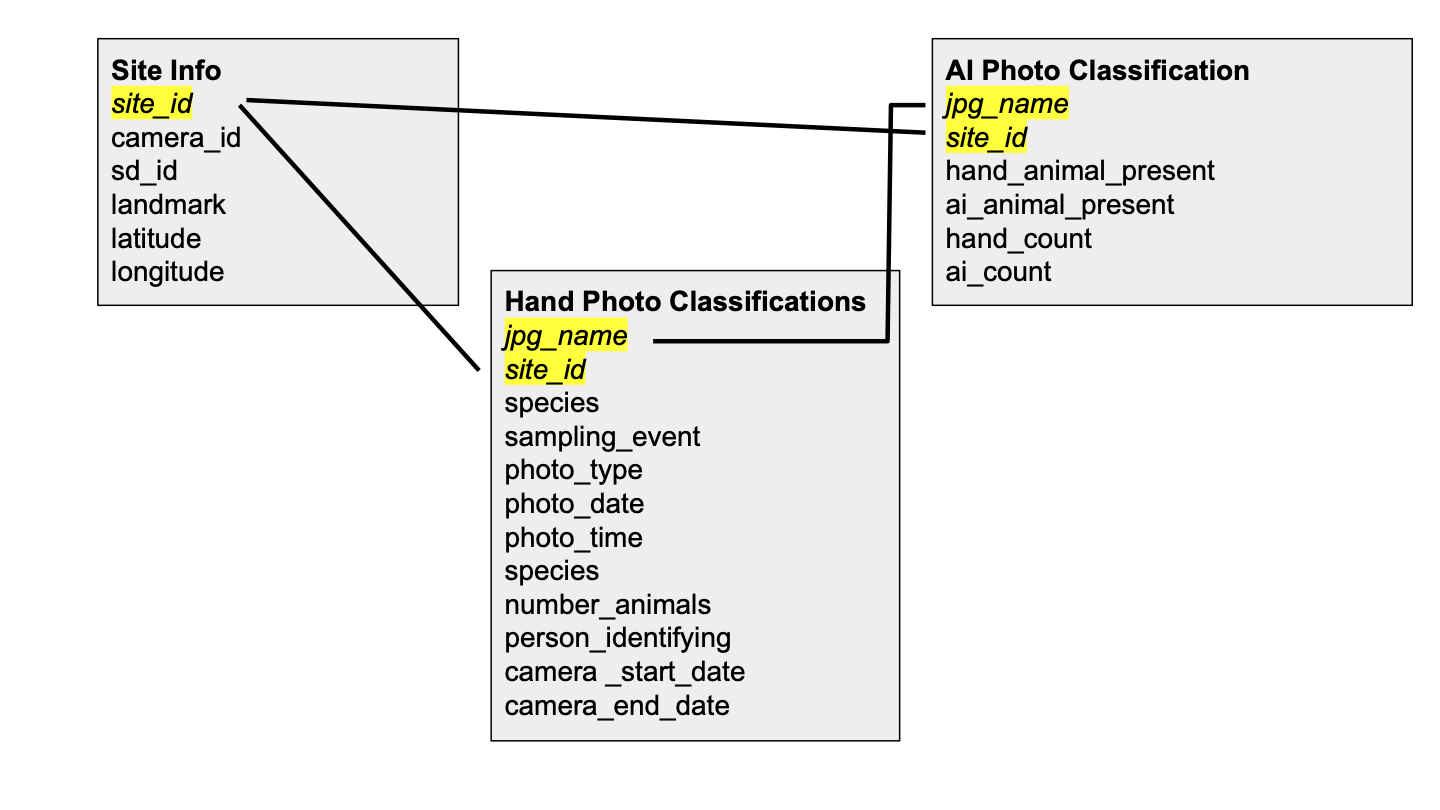
\includegraphics[width=13.33in]{/Users/courtney/Desktop/MS_Thesis/R-Code/Count_Check_Bookdown/Database_Structure_Diagram} \end{center}

The highlighted items are the primary and foreign keys for each dataframe. The black lines show how the foreign keys will connect the dataframes to each other.

Site\_id is the primary key for the site info, since each row contains info on a unique site, and it can also be used as foreign key to link it to the count dataframes. Jpeg\_name is the primary key for both count dataframes, because of their rows contain data for a single unique jpg. Jpeg\_name can also serve as a foreign key to connect the count dataframes to each other, since both dataframes contain info on the same set of jpegs.

\hypertarget{getting-necessary-packages}{%
\section{Getting Necessary Packages}\label{getting-necessary-packages}}

\hypertarget{install-dbi}{%
\subsection{Install DBI}\label{install-dbi}}

I am trying to install a database in SQL, so I will need the \texttt{DBI} package.

\begin{Shaded}
\begin{Highlighting}[]
\FunctionTok{install.packages}\NormalTok{(}\StringTok{"RSQLite"}\NormalTok{)}
\FunctionTok{install.packages}\NormalTok{(}\StringTok{"DBI"}\NormalTok{)}
\end{Highlighting}
\end{Shaded}

\hypertarget{calling-packages-into-r}{%
\subsection{Calling packages into R}\label{calling-packages-into-r}}

In addition to loading \texttt{DBI}, I also need \texttt{tidyverse} and \texttt{lubridate} to clean the data.

\begin{Shaded}
\begin{Highlighting}[]
\FunctionTok{library}\NormalTok{(DBI)}
\FunctionTok{library}\NormalTok{(tidyverse)}
\FunctionTok{library}\NormalTok{(lubridate)}
\end{Highlighting}
\end{Shaded}

\hypertarget{load-the-data}{%
\section{Load the Data}\label{load-the-data}}

The full database of all the AI and hand counted photos is apparently too big to work with as just 2 files, so I have subsetted it into seasons. I have included just one season/year (summer 2019) to show my process in a way that doesn't have too much repetition, though it works them same for all the season/years.

I am loading three csvs: the hand counts of deer, the ai counts of deer, and the information on each site.

\begin{Shaded}
\begin{Highlighting}[]
\NormalTok{hand }\OtherTok{\textless{}{-}} \FunctionTok{read.csv}\NormalTok{(}\StringTok{"/Users/courtney/Desktop/MS\_Thesis/Data/Compiled{-}Raw/summer19.csv"}\NormalTok{, }\AttributeTok{stringsAsFactors =} \ConstantTok{FALSE}\NormalTok{)}

\NormalTok{ai }\OtherTok{\textless{}{-}} \FunctionTok{read.csv}\NormalTok{(}\StringTok{"/Users/courtney/Desktop/MS\_Thesis/Data/Compiled{-}Raw/AI.summer19.csv"}\NormalTok{, }\AttributeTok{stringsAsFactors =} \ConstantTok{FALSE}\NormalTok{)}

\NormalTok{site }\OtherTok{\textless{}{-}} \FunctionTok{read.csv}\NormalTok{(}\StringTok{"/Users/courtney/Desktop/MS\_Thesis/Data/Compiled{-}Raw/site\_info.csv"}\NormalTok{, }\AttributeTok{stringsAsFactors =} \ConstantTok{FALSE}\NormalTok{)}
\end{Highlighting}
\end{Shaded}

\hypertarget{clean-the-data}{%
\section{Clean the Data}\label{clean-the-data}}

First, I clean the hand count data. To do this, I coerce the photo date/photo time columns to be date and time objects, respectively. I also pull out only the columns I want, to leave out redundant categories like organism family, order, class, etc. and rename them so that common columns/keys will match with the other dataframes.

\begin{Shaded}
\begin{Highlighting}[]
\NormalTok{hand.clean }\OtherTok{\textless{}{-}}\NormalTok{ hand }\SpecialCharTok{\%\textgreater{}\%} 
  \FunctionTok{mutate}\NormalTok{(}\AttributeTok{dt =} \FunctionTok{ymd\_hms}\NormalTok{(}\FunctionTok{paste}\NormalTok{(Photo.Date, Photo.time))) }\SpecialCharTok{\%\textgreater{}\%} 
  \FunctionTok{select}\NormalTok{(}\AttributeTok{jpg\_name =}\NormalTok{ Raw.Name,}
         \AttributeTok{site\_id =}\NormalTok{ Camera.Trap.Name,}
         \AttributeTok{species =}\NormalTok{ Species,}
         \AttributeTok{sampling\_event =}\NormalTok{ Sampling.Event,}
         \AttributeTok{photo\_type =}\NormalTok{ Photo.Type,}
         \AttributeTok{photo\_date =}\NormalTok{ Photo.Date,}
         \AttributeTok{photo\_time =}\NormalTok{ Photo.time,}
         \AttributeTok{n\_all =}\NormalTok{ Number.of.Animals,}
         \AttributeTok{person\_identifying =}\NormalTok{ Person.Identifying.the.Photo,}
         \AttributeTok{camera\_start\_date =}\NormalTok{ Camera.Start.Date,}
         \AttributeTok{camera\_end\_date =}\NormalTok{ Camera.End.Date) }\SpecialCharTok{\%\textgreater{}\%} 
  \CommentTok{\# Mule deer are tagged with species as \textquotesingle{}hemionus\textquotesingle{}}
  \FunctionTok{mutate}\NormalTok{(}\AttributeTok{n\_animals =} \FunctionTok{case\_when}\NormalTok{(}
\NormalTok{    species }\SpecialCharTok{==} \StringTok{"hemionus"} \SpecialCharTok{|}\NormalTok{ species }\SpecialCharTok{==} \StringTok{"guttata"} \SpecialCharTok{\textasciitilde{}}\NormalTok{ n\_all,}
    \ConstantTok{TRUE} \SpecialCharTok{\textasciitilde{}}\NormalTok{ 0L}
\NormalTok{  )) }\SpecialCharTok{\%\textgreater{}\%} 
  \CommentTok{\# Drop n\_animals and species}
  \FunctionTok{select}\NormalTok{(}\SpecialCharTok{{-}}\NormalTok{n\_all)}
\end{Highlighting}
\end{Shaded}

Next, I clean the AI count data. Once again, I pull out only the columns I want and leave out extra unnccessary columns like the file path to the jpg, etc. and rename them so that common columns/keys will match with the other dataframes.

\begin{Shaded}
\begin{Highlighting}[]
\NormalTok{ai.clean }\OtherTok{\textless{}{-}}\NormalTok{ ai }\SpecialCharTok{\%\textgreater{}\%} 
  \FunctionTok{select}\NormalTok{(}\AttributeTok{jpg\_name =}\NormalTok{ Raw\_Name,}
         \AttributeTok{site\_id =}\NormalTok{ Camera.Trap.Name,}
         \AttributeTok{hand\_animal\_present =}\NormalTok{ hand\_label\_has\_animal,}
         \AttributeTok{ai\_animal\_present =}\NormalTok{ det\_has\_animal,}
         \AttributeTok{ai\_count =}\NormalTok{ n\_pred\_deer)}
\end{Highlighting}
\end{Shaded}

Lastly, I do modify the ``site\_id'' category so that it is consistent across all three databases. Because the ``site'' dataframe just includes site as a single number, I remove all the ``SITE'' characters from the hand count and AI count dataframes.

\begin{Shaded}
\begin{Highlighting}[]
\NormalTok{hand.clean}\SpecialCharTok{$}\NormalTok{site\_id }\OtherTok{=} \FunctionTok{gsub}\NormalTok{(}\StringTok{" "}\NormalTok{, }\StringTok{""}\NormalTok{, hand.clean}\SpecialCharTok{$}\NormalTok{site\_id)}
\NormalTok{hand.clean}\SpecialCharTok{$}\NormalTok{site\_id }\OtherTok{=} \FunctionTok{gsub}\NormalTok{(}\StringTok{"Site"}\NormalTok{, }\StringTok{""}\NormalTok{, hand.clean}\SpecialCharTok{$}\NormalTok{site\_id)}

\NormalTok{ai.clean}\SpecialCharTok{$}\NormalTok{site\_id }\OtherTok{=} \FunctionTok{gsub}\NormalTok{(}\StringTok{"site"}\NormalTok{, }\StringTok{""}\NormalTok{, ai.clean}\SpecialCharTok{$}\NormalTok{site\_id)}
\NormalTok{ai.clean}\SpecialCharTok{$}\NormalTok{site\_id }\OtherTok{=} \FunctionTok{gsub}\NormalTok{(}\StringTok{"00"}\NormalTok{, }\StringTok{""}\NormalTok{, ai.clean}\SpecialCharTok{$}\NormalTok{site\_id)}
\NormalTok{ai.clean}\SpecialCharTok{$}\NormalTok{site\_id }\OtherTok{=} \FunctionTok{gsub}\NormalTok{(}\StringTok{"(?\textless{}!}\SpecialCharTok{\textbackslash{}\textbackslash{}}\StringTok{d)0"}\NormalTok{, }\StringTok{""}\NormalTok{, ai.clean}\SpecialCharTok{$}\NormalTok{site\_id, }\AttributeTok{perl =} \ConstantTok{TRUE}\NormalTok{)}
\end{Highlighting}
\end{Shaded}

\hypertarget{create-a-new-empty-sql-database}{%
\section{Create a New, Empty SQL Database}\label{create-a-new-empty-sql-database}}

Here, I create an empty SQL database using the DBI package that I can later populate.

\begin{Shaded}
\begin{Highlighting}[]
\NormalTok{counts\_db }\OtherTok{\textless{}{-}} \FunctionTok{dbConnect}\NormalTok{(RSQLite}\SpecialCharTok{::}\FunctionTok{SQLite}\NormalTok{(), }\StringTok{"/Users/courtney/Desktop/MS\_Thesis/Data/SQL\_db.db"}\NormalTok{)}
\end{Highlighting}
\end{Shaded}

\hypertarget{append-the-cleaned-data-to-the-empty-sql-database}{%
\section{Append the Cleaned Data to the Empty SQL Database}\label{append-the-cleaned-data-to-the-empty-sql-database}}

First, I create the database tables, specificing the primary and foreign keys for each one.

\textbf{Site Info Table:}

\begin{Shaded}
\begin{Highlighting}[]
\FunctionTok{dbExecute}\NormalTok{(counts\_db, }
\StringTok{"CREATE TABLE site\_info (}
\StringTok{ site\_id double(3) NOT NULL,}
\StringTok{ camera\_id double(3) NOT NULL,}
\StringTok{ sd\_id varchar(5) NOT NULL,}
\StringTok{ lat double(20),}
\StringTok{ long double(20),}
\StringTok{ mount char(100),}
\StringTok{ landmark   char(100),}
\StringTok{ PRIMARY KEY (site\_id)}
\StringTok{);"}\NormalTok{)}
\end{Highlighting}
\end{Shaded}

\textbf{AI Count Table:}

\begin{Shaded}
\begin{Highlighting}[]
\FunctionTok{dbExecute}\NormalTok{(counts\_db, }
\StringTok{"CREATE TABLE ai\_counts (}
\StringTok{ jpg\_name varchar(100) NOT NULL,}
\StringTok{ site\_id double(3) NOT NULL,}
\StringTok{ hand\_animal\_present char(10),}
\StringTok{ ai\_animal\_present char(10),}
\StringTok{ ai\_count double(10),}
\StringTok{ PRIMARY KEY (jpg\_name)}
\StringTok{ FOREIGN KEY (jpg\_name) REFERENCES hand\_counts(jpg\_name)}
\StringTok{ FOREIGN KEY (site\_id) REFERENCES site\_info(site\_id)}
\StringTok{);"}\NormalTok{)}
\end{Highlighting}
\end{Shaded}

\textbf{Hand Count Table:}

\begin{Shaded}
\begin{Highlighting}[]
\FunctionTok{dbExecute}\NormalTok{(counts\_db, }
\StringTok{"CREATE TABLE hand\_counts (}
\StringTok{ jpg\_name varchar(100) NOT NULL,}
\StringTok{ site\_id double(3) NOT NULL,}
\StringTok{ species char(50),}
\StringTok{ sampling\_event varchar(50),}
\StringTok{ photo\_type varchar(50),}
\StringTok{ photo\_date varchar(50),}
\StringTok{ photo\_time varchar(50),}
\StringTok{ person\_identifying varchar(50),}
\StringTok{ camera\_start\_date varchar(50),}
\StringTok{ camera\_end\_date varchar(50),}
\StringTok{ n\_animals double(10),}
\StringTok{ PRIMARY KEY (jpg\_name)}
\StringTok{ FOREIGN KEY (jpg\_name) REFERENCES ai\_counts(jpg\_name)}
\StringTok{ FOREIGN KEY (site\_id) REFERENCES site\_info(site\_id)}
\StringTok{);"}\NormalTok{)}
\end{Highlighting}
\end{Shaded}

Then, I add all of the cleaned dataframes into the SQL database. Database complete! I also check to make sure that the dataframes were actually added by calling their first ten rows to look at.

\begin{Shaded}
\begin{Highlighting}[]
\FunctionTok{dbWriteTable}\NormalTok{(counts\_db, }\StringTok{"site\_info"}\NormalTok{, site, }\AttributeTok{append =} \ConstantTok{TRUE}\NormalTok{)}
\FunctionTok{dbGetQuery}\NormalTok{(counts\_db, }\StringTok{"SELECT * FROM site\_info LIMIT 10;"}\NormalTok{)}

\FunctionTok{dbWriteTable}\NormalTok{(counts\_db, }\StringTok{"ai\_counts"}\NormalTok{, ai.clean, }\AttributeTok{append =} \ConstantTok{TRUE}\NormalTok{)}
\FunctionTok{dbGetQuery}\NormalTok{(counts\_db, }\StringTok{"SELECT * FROM ai\_counts LIMIT 10;"}\NormalTok{)}

\FunctionTok{dbWriteTable}\NormalTok{(counts\_db, }\StringTok{"hand\_counts"}\NormalTok{, hand.clean, }\AttributeTok{append =} \ConstantTok{TRUE}\NormalTok{)}
\FunctionTok{dbGetQuery}\NormalTok{(counts\_db, }\StringTok{"SELECT * FROM hand\_counts LIMIT 10;"}\NormalTok{)}
\end{Highlighting}
\end{Shaded}

\hypertarget{overall}{%
\chapter{Checking Overall Agreement}\label{overall}}

First, I want to get a sense of the overall agreement between hand counts and AI counts. This will give an idea of the total amount of data we might be losing to the AI algorithm. To do this, I first have to calculate the difference between the AI and hand counts.

\begin{Shaded}
\begin{Highlighting}[]
\NormalTok{hand.counts }\OtherTok{\textless{}{-}} \FunctionTok{dbGetQuery}\NormalTok{(counts\_db, }\StringTok{"SELECT * FROM hand\_counts;"}\NormalTok{)}
\NormalTok{ai.counts }\OtherTok{\textless{}{-}} \FunctionTok{dbGetQuery}\NormalTok{(counts\_db, }\StringTok{"SELECT * FROM ai\_counts;"}\NormalTok{)}

\NormalTok{ai\_hand }\OtherTok{\textless{}{-}}\NormalTok{ hand.counts }\SpecialCharTok{\%\textgreater{}\%} 
  \FunctionTok{inner\_join}\NormalTok{(ai.counts, }\AttributeTok{by =} \FunctionTok{c}\NormalTok{(}\StringTok{"jpg\_name"}\NormalTok{, }\StringTok{"site\_id"}\NormalTok{)) }\SpecialCharTok{\%\textgreater{}\%}
  \FunctionTok{mutate}\NormalTok{(}\AttributeTok{diff =}\NormalTok{ n\_animals }\SpecialCharTok{{-}}\NormalTok{ ai\_count)}
\end{Highlighting}
\end{Shaded}

Next, I look at the \emph{mean}, \emph{standard deviation}, and \emph{range} of difference between AI and hand counts.

\begin{Shaded}
\begin{Highlighting}[]
\NormalTok{m }\OtherTok{=} \FunctionTok{mean}\NormalTok{(ai\_hand}\SpecialCharTok{$}\NormalTok{diff)}
\NormalTok{s }\OtherTok{=} \FunctionTok{sd}\NormalTok{(ai\_hand}\SpecialCharTok{$}\NormalTok{diff)}
\NormalTok{r }\OtherTok{=} \FunctionTok{range}\NormalTok{(ai\_hand}\SpecialCharTok{$}\NormalTok{diff)}
\end{Highlighting}
\end{Shaded}

Here's the \textbf{Mean}:

\begin{verbatim}
## [1] 0.005713605
\end{verbatim}

Here's the \textbf{Standard Deviation}:

\begin{verbatim}
## [1] 0.1933531
\end{verbatim}

Here's the \textbf{Range}:

\begin{verbatim}
## [1] -4  8
\end{verbatim}

From this, I can see that the mean and sd are very low, but the range shows that there are still some pretty big miscounts by the AI. So I also want to check how often the AI makes ``big'' miscalculations. ``Big'' in this case, is any instance of \textgreater{} +/-1 deer.

\begin{Shaded}
\begin{Highlighting}[]
\NormalTok{ai\_hand }\SpecialCharTok{\%\textgreater{}\%} 
  \FunctionTok{group\_by}\NormalTok{(diff) }\SpecialCharTok{\%\textgreater{}\%} 
  \FunctionTok{summarize}\NormalTok{(}\AttributeTok{freq =} \FunctionTok{n}\NormalTok{()) }\SpecialCharTok{\%\textgreater{}\%}
  \FunctionTok{mutate}\NormalTok{(}\AttributeTok{percent =} \FunctionTok{round}\NormalTok{((freq}\SpecialCharTok{/}\FunctionTok{sum}\NormalTok{(freq)}\SpecialCharTok{*}\DecValTok{100}\NormalTok{))) }\SpecialCharTok{\%\textgreater{}\%}
  \FunctionTok{rename}\NormalTok{(}\StringTok{"Count Difference"} \OtherTok{=}\NormalTok{ diff,}
         \StringTok{"Frequency"} \OtherTok{=}\NormalTok{ freq,}
         \StringTok{"Percent of Observations"} \OtherTok{=}\NormalTok{ percent) }\SpecialCharTok{\%\textgreater{}\%}
\NormalTok{  knitr}\SpecialCharTok{::}\FunctionTok{kable}\NormalTok{(}\AttributeTok{align =} \StringTok{"c"}\NormalTok{) }
\end{Highlighting}
\end{Shaded}

\begin{tabular}{c|c|c}
\hline
Count Difference & Frequency & Percent of Observations\\
\hline
-4 & 1 & 0\\
\hline
-3 & 7 & 0\\
\hline
-2 & 47 & 0\\
\hline
-1 & 1399 & 1\\
\hline
0 & 130883 & 97\\
\hline
1 & 1604 & 1\\
\hline
2 & 250 & 0\\
\hline
3 & 39 & 0\\
\hline
4 & 4 & 0\\
\hline
5 & 1 & 0\\
\hline
6 & 2 & 0\\
\hline
7 & 1 & 0\\
\hline
8 & 3 & 0\\
\hline
\end{tabular}

Looks like most of the AI's counts are within the +/-1 deer range! The big miscounts make up only less than one percent of the counts.

Overall, agreement seems pretty good! The mean and sd are very low, and even though there some big miscounts, they are a very small portion of all the counts.

\hypertarget{site}{%
\chapter{Checking Site-level Agreement}\label{site}}

Even though overall agreement is really good, it's possible that there are some sites where the AI is less effective because of the terrain, shade level, etc. Because our sites don't change, if I identify problem sites now, I can know to not trust the AI's counts and to hand--count these sites in the future.

First things first: I want to check the min, max, and mean of count difference for each site.

\begin{Shaded}
\begin{Highlighting}[]
\NormalTok{site\_diff }\OtherTok{\textless{}{-}}\NormalTok{ ai\_hand }\SpecialCharTok{\%\textgreater{}\%} 
  \FunctionTok{group\_by}\NormalTok{(site\_id) }\SpecialCharTok{\%\textgreater{}\%} 
  \FunctionTok{summarize}\NormalTok{(}\AttributeTok{n =} \FunctionTok{n}\NormalTok{(),}
            \AttributeTok{min\_diff =} \FunctionTok{min}\NormalTok{(diff),}
            \AttributeTok{mean\_diff =} \FunctionTok{mean}\NormalTok{(diff),}
            \AttributeTok{max\_diff =} \FunctionTok{max}\NormalTok{(diff))}

\NormalTok{site\_diff }\SpecialCharTok{\%\textgreater{}\%}
  \FunctionTok{arrange}\NormalTok{(}\FunctionTok{desc}\NormalTok{(max\_diff)) }\SpecialCharTok{\%\textgreater{}\%}
  \FunctionTok{slice\_head}\NormalTok{(}\AttributeTok{n =} \DecValTok{20}\NormalTok{) }\SpecialCharTok{\%\textgreater{}\%}
  \FunctionTok{rename}\NormalTok{(}\AttributeTok{Site =}\NormalTok{ site\_id,}
         \StringTok{"Number of Observations"} \OtherTok{=}\NormalTok{ n,}
         \AttributeTok{Min\_Diff =}\NormalTok{ min\_diff,}
         \AttributeTok{Mean\_Diff =}\NormalTok{ mean\_diff,}
         \AttributeTok{Max\_Diff =}\NormalTok{ max\_diff) }\SpecialCharTok{\%\textgreater{}\%}
\NormalTok{  knitr}\SpecialCharTok{::}\FunctionTok{kable}\NormalTok{(}\AttributeTok{align =} \StringTok{"c"}\NormalTok{)}
\end{Highlighting}
\end{Shaded}

\begin{tabular}{c|c|c|c|c}
\hline
Site & Number of Observations & Min\_Diff & Mean\_Diff & Max\_Diff\\
\hline
74 & 1585 & -3 & 0.1249211 & 8\\
\hline
8 & 312 & -2 & 0.1089744 & 3\\
\hline
41 & 14694 & -4 & 0.0596162 & 3\\
\hline
68 & 946 & 0 & 0.0528541 & 3\\
\hline
82 & 191 & -1 & 0.1413613 & 3\\
\hline
86 & 2224 & -1 & 0.0193345 & 3\\
\hline
25 & 11352 & -1 & -0.0069591 & 2\\
\hline
40 & 2112 & -1 & -0.0066288 & 2\\
\hline
42 & 2229 & -2 & -0.0116644 & 2\\
\hline
44 & 4905 & -3 & -0.0101937 & 2\\
\hline
75 & 1812 & -1 & -0.0005519 & 2\\
\hline
79 & 2828 & -1 & 0.0042433 & 2\\
\hline
87 & 2582 & -1 & 0.0290473 & 2\\
\hline
90 & 2379 & -1 & 0.0369903 & 2\\
\hline
98 & 1234 & -1 & -0.0008104 & 2\\
\hline
1 & 622 & -1 & 0.0209003 & 1\\
\hline
5 & 171 & -1 & 0.0175439 & 1\\
\hline
7 & 489 & -1 & -0.0020450 & 1\\
\hline
9 & 4666 & -3 & -0.0025718 & 1\\
\hline
10 & 3546 & -1 & -0.0016920 & 1\\
\hline
\end{tabular}

Definitely a lot of variation! Some sites are perfect, others are in between, and one site (Site 74) has the biggest over-count AND nearly the biggest under-count. To help better get a grasp of the variation, I'm going to plot it by site.

\begin{Shaded}
\begin{Highlighting}[]
\NormalTok{site\_diff }\SpecialCharTok{\%\textgreater{}\%}
  \FunctionTok{arrange}\NormalTok{(}\FunctionTok{desc}\NormalTok{(site\_id)) }\SpecialCharTok{\%\textgreater{}\%}
  \FunctionTok{ggplot}\NormalTok{(}\FunctionTok{aes}\NormalTok{(}\AttributeTok{x =} \FunctionTok{factor}\NormalTok{(site\_id), }\AttributeTok{y =}\NormalTok{ mean\_diff)) }\SpecialCharTok{+}
  \FunctionTok{geom\_point}\NormalTok{() }\SpecialCharTok{+}
  \FunctionTok{geom\_errorbar}\NormalTok{(}\FunctionTok{aes}\NormalTok{(}\AttributeTok{ymin =}\NormalTok{ min\_diff, }\AttributeTok{ymax =}\NormalTok{ max\_diff)) }\SpecialCharTok{+}
  \FunctionTok{labs}\NormalTok{(}\AttributeTok{title =} \StringTok{"Comparison of AI Counts to Hand Counts by Site"}\NormalTok{, }\AttributeTok{x =} \StringTok{"Site"}\NormalTok{, }\AttributeTok{y =} \StringTok{"Difference (Hand {-} AI)"}\NormalTok{) }\SpecialCharTok{+}
  \FunctionTok{theme\_light}\NormalTok{() }\SpecialCharTok{+}
  \FunctionTok{theme}\NormalTok{(}\AttributeTok{plot.title =} \FunctionTok{element\_text}\NormalTok{(}\AttributeTok{size =} \DecValTok{19}\NormalTok{, }\AttributeTok{face =} \StringTok{"bold"}\NormalTok{, }\AttributeTok{hjust =} \FloatTok{0.5}\NormalTok{),}
        \AttributeTok{axis.title =} \FunctionTok{element\_text}\NormalTok{(}\AttributeTok{size =} \DecValTok{11}\NormalTok{),}
        \AttributeTok{axis.text.x =} \FunctionTok{element\_text}\NormalTok{(}\AttributeTok{size =} \DecValTok{7}\NormalTok{, }\AttributeTok{angle =} \DecValTok{90}\NormalTok{, }\AttributeTok{vjust =} \FloatTok{0.5}\NormalTok{))}
\end{Highlighting}
\end{Shaded}

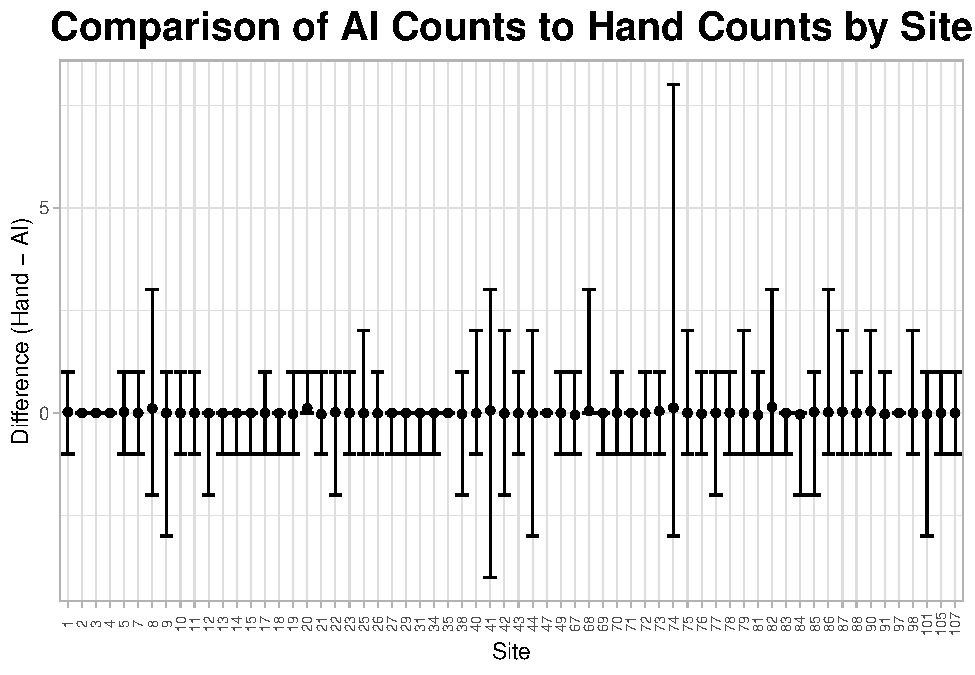
\includegraphics{Count_Check_Bookdown_files/figure-latex/plot_diffs-1.pdf}

While this is a good eyeball assessment, I want to firmly identify ``problem'' sites. A ``problem'' site in this case is going to be defined as any site that correctly counts \textless90\% of all photos.

\begin{Shaded}
\begin{Highlighting}[]
\NormalTok{ai\_hand }\SpecialCharTok{\%\textgreater{}\%} 
  \FunctionTok{group\_by}\NormalTok{(site\_id, diff) }\SpecialCharTok{\%\textgreater{}\%}
  \FunctionTok{summarize}\NormalTok{(}\AttributeTok{freq =} \FunctionTok{n}\NormalTok{()) }\SpecialCharTok{\%\textgreater{}\%}
  \FunctionTok{mutate}\NormalTok{(}\AttributeTok{percent =} \FunctionTok{round}\NormalTok{((freq}\SpecialCharTok{/}\FunctionTok{sum}\NormalTok{(freq)}\SpecialCharTok{*}\DecValTok{100}\NormalTok{), }\AttributeTok{digits =} \DecValTok{2}\NormalTok{) ) }\SpecialCharTok{\%\textgreater{}\%}
  \FunctionTok{filter}\NormalTok{(}\FunctionTok{max}\NormalTok{(percent) }\SpecialCharTok{\textless{}} \DecValTok{90}\NormalTok{) }\SpecialCharTok{\%\textgreater{}\%}
  \FunctionTok{top\_n}\NormalTok{(}\DecValTok{1}\NormalTok{, percent) }\SpecialCharTok{\%\textgreater{}\%}
  \FunctionTok{select}\NormalTok{(site\_id, percent) }\SpecialCharTok{\%\textgreater{}\%}
  \FunctionTok{rename}\NormalTok{(}\AttributeTok{Site =}\NormalTok{ site\_id,}
         \StringTok{"Percent Correct AI Counts"} \OtherTok{=}\NormalTok{ percent) }\SpecialCharTok{\%\textgreater{}\%}
\NormalTok{  knitr}\SpecialCharTok{::}\FunctionTok{kable}\NormalTok{(}\AttributeTok{align =} \StringTok{"c"}\NormalTok{) }
\end{Highlighting}
\end{Shaded}

\begin{tabular}{c|c}
\hline
Site & Percent Correct AI Counts\\
\hline
8 & 77.88\\
\hline
20 & 88.89\\
\hline
74 & 87.95\\
\hline
82 & 89.01\\
\hline
\end{tabular}

Only four sites! That's not bad. And most of them hover around 90\% agreement, with only one site (Site 8) sporting a truly abysmal 77.88\% agreement. Now that I know these sites are difficult for the AI to count deer at, I can be sure to check their counts by hand going forward.

\hypertarget{conclusion}{%
\chapter{Conclusion}\label{conclusion}}

Overall, the AI seems to perform pretty well! While there are a handful of sites that will still need to be hand-counted, the AI will still be able to save us a lot of time without sacrificing much data! Yay!

\begin{center}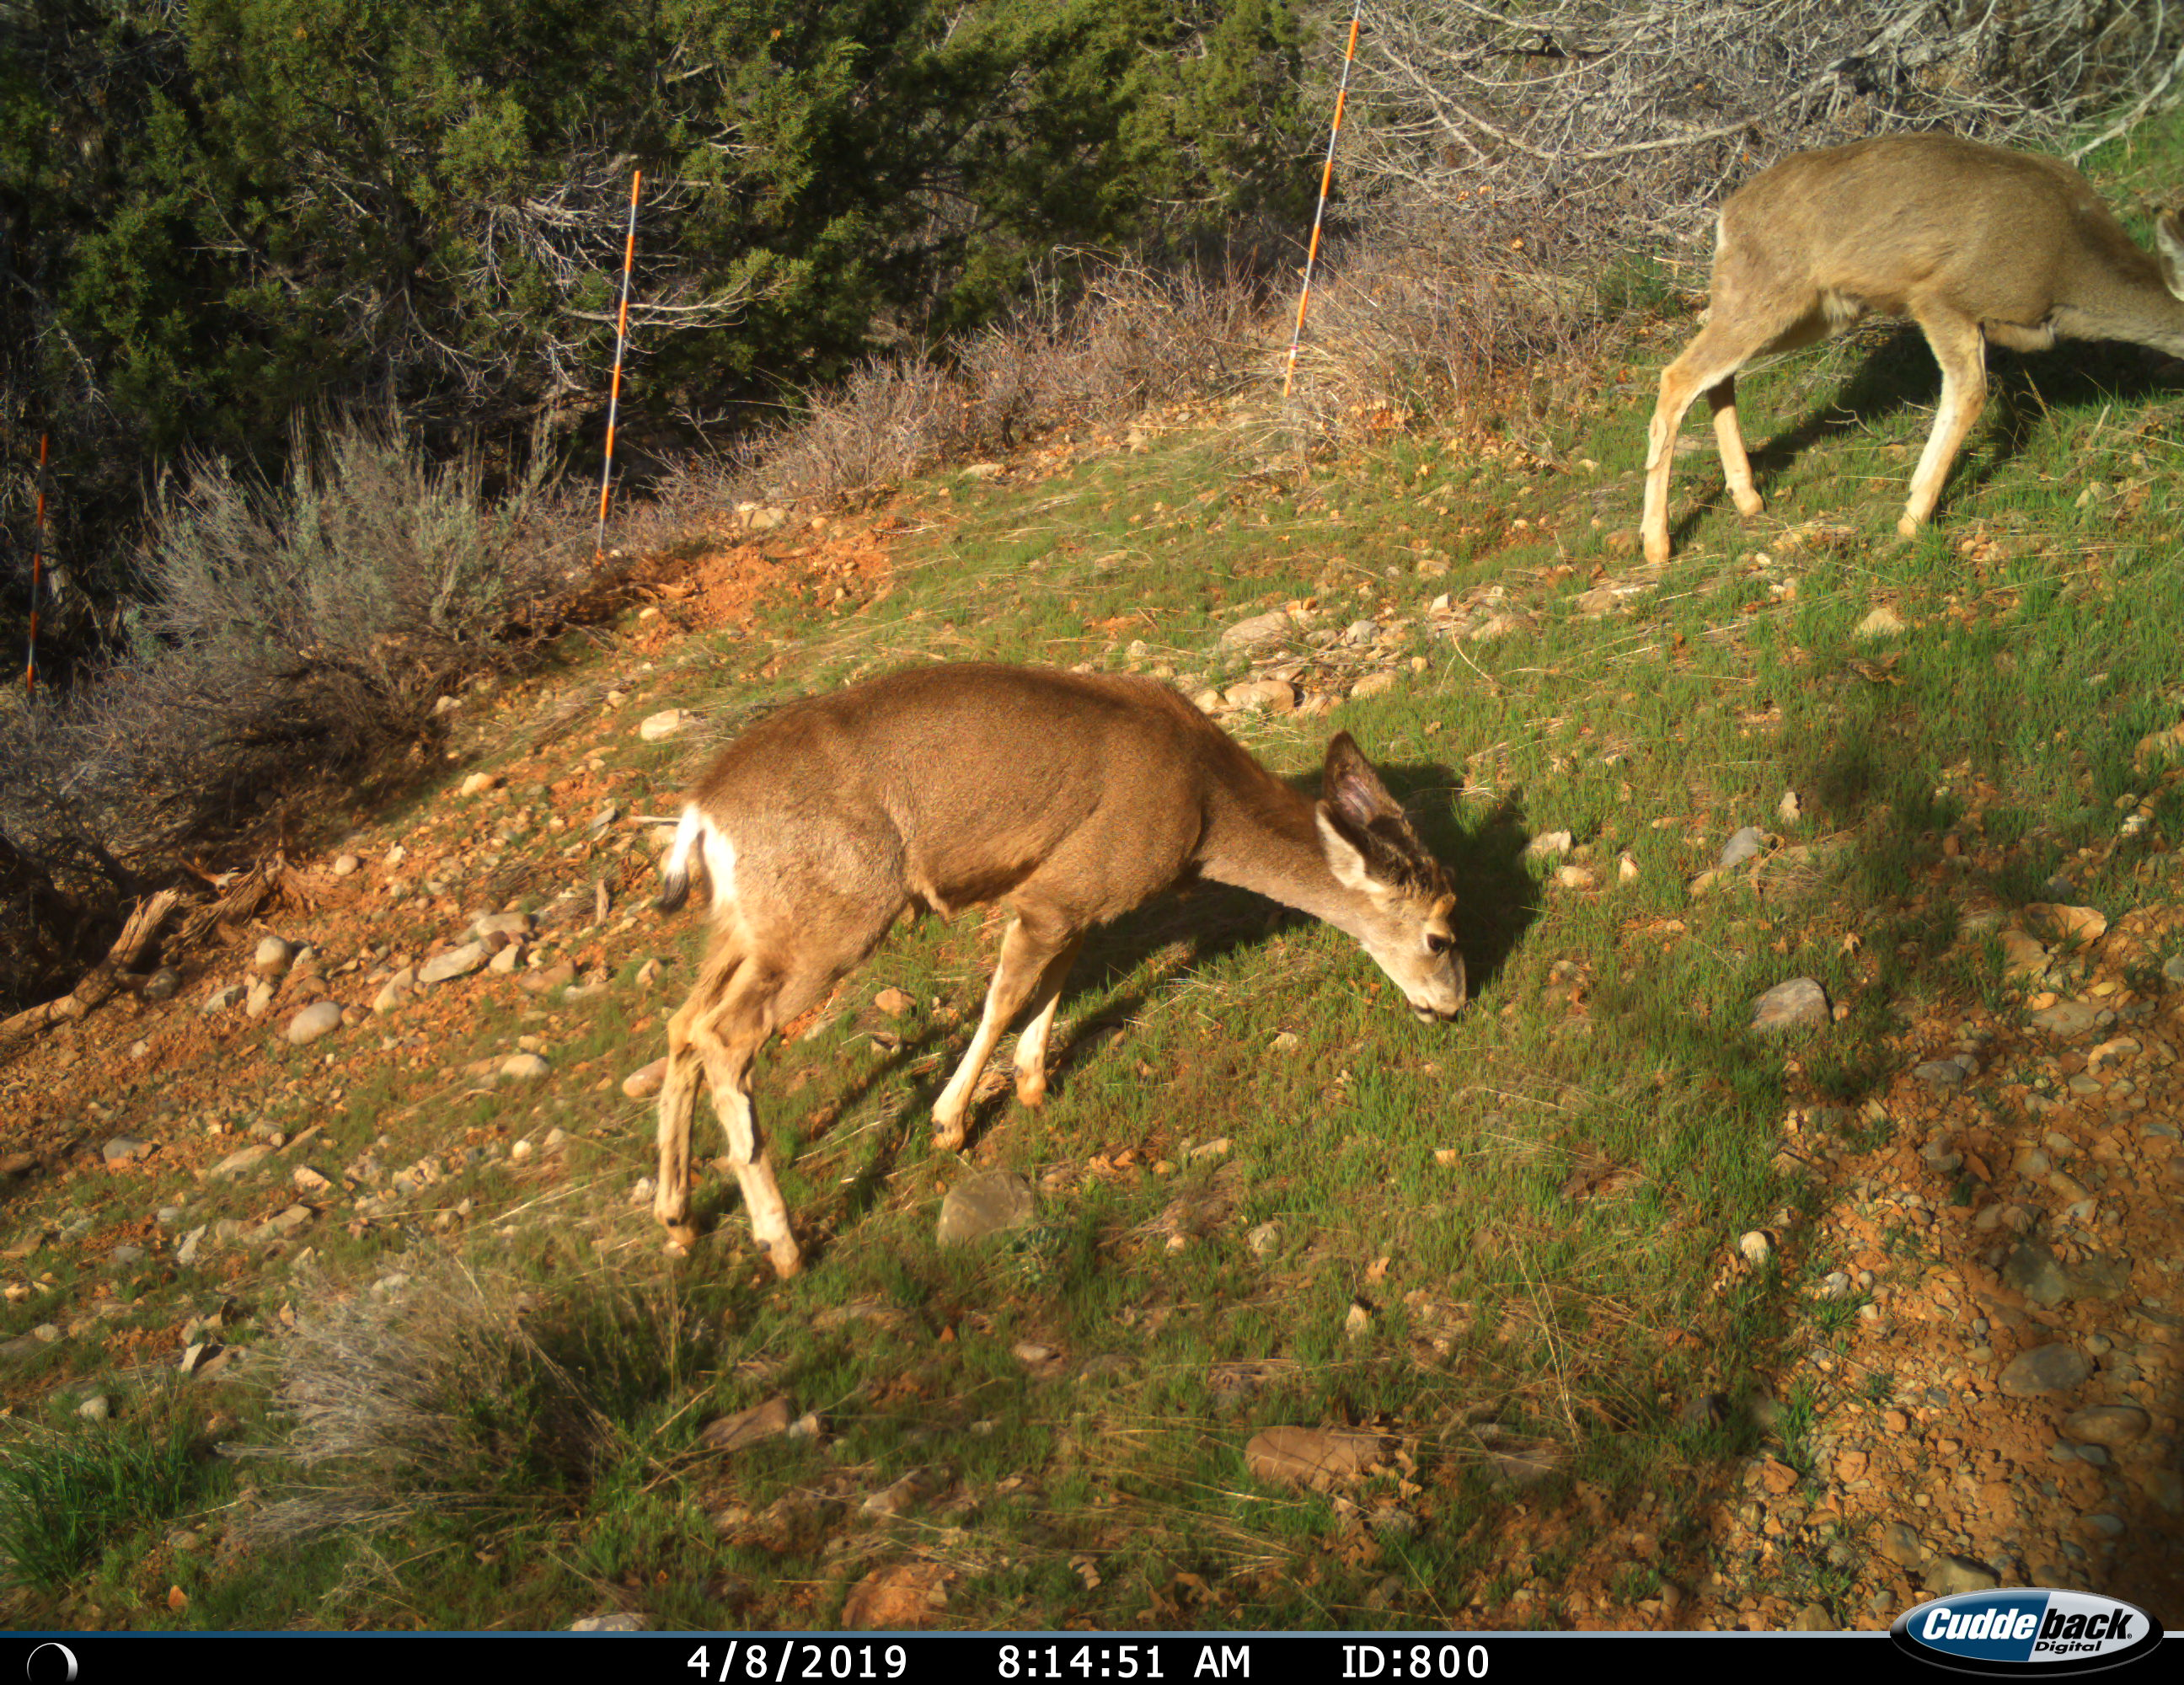
\includegraphics[width=36in]{/Users/courtney/Desktop/MS_Thesis/R-Code/Count_Check_Bookdown/site002_sd008_spring2019_72} \end{center}

  \bibliography{book.bib,packages.bib}

\end{document}
